\documentclass[a4paper]{article}

\def\npart {III}
\def\nterm {Lent}
\def\nyear {2017}
\def\nlecturer {B. P. Narayanan}
\def\ncourse {Ramsey Theory}

% Imports
\ifx \nextra \undefined
  \usepackage[pdftex,
    hidelinks,
    pdfauthor={Dexter Chua},
    pdfsubject={Cambridge Maths Notes: Part \npart\ - \ncourse},
    pdftitle={Part \npart\ - \ncourse},
  pdfkeywords={Cambridge Mathematics Maths Math \npart\ \nterm\ \nyear\ \ncourse}]{hyperref}
  \title{Part \npart\ - \ncourse}
\else
  \usepackage[pdftex,
    hidelinks,
    pdfauthor={Dexter Chua},
    pdfsubject={Cambridge Maths Notes: Part \npart\ - \ncourse\ (\nextra)},
    pdftitle={Part \npart\ - \ncourse\ (\nextra)},
  pdfkeywords={Cambridge Mathematics Maths Math \npart\ \nterm\ \nyear\ \ncourse\ \nextra}]{hyperref}

  \title{Part \npart\ - \ncourse \\ {\Large \nextra}}
\fi

\author{Lectured by \nlecturer \\\small Notes taken by Dexter Chua}
\date{\nterm\ \nyear}

\usepackage{alltt}
\usepackage{amsfonts}
\usepackage{amsmath}
\usepackage{amssymb}
\usepackage{amsthm}
\usepackage{booktabs}
\usepackage{caption}
\usepackage{enumitem}
\usepackage{fancyhdr}
\usepackage{graphicx}
\usepackage{mathtools}
\usepackage{microtype}
\usepackage{multirow}
\usepackage{pdflscape}
\usepackage{pgfplots}
\usepackage{siunitx}
\usepackage{tabularx}
\usepackage{tikz}
\usepackage{tkz-euclide}
\usepackage[normalem]{ulem}
\usepackage[all]{xy}

\pgfplotsset{compat=1.12}

\pagestyle{fancyplain}
\lhead{\emph{\nouppercase{\leftmark}}}
\ifx \nextra \undefined
  \rhead{
    \ifnum\thepage=1
    \else
      \npart\ \ncourse
    \fi}
\else
  \rhead{
    \ifnum\thepage=1
    \else
      \npart\ \ncourse\ (\nextra)
    \fi}
\fi
\usetikzlibrary{arrows}
\usetikzlibrary{decorations.markings}
\usetikzlibrary{decorations.pathmorphing}
\usetikzlibrary{positioning}
\usetikzlibrary{fadings}
\usetikzlibrary{intersections}
\usetikzlibrary{cd}

\newcommand*{\Cdot}{\raisebox{-0.25ex}{\scalebox{1.5}{$\cdot$}}}
\newcommand {\pd}[2][ ]{
  \ifx #1 { }
    \frac{\partial}{\partial #2}
  \else
    \frac{\partial^{#1}}{\partial #2^{#1}}
  \fi
}

% Theorems
\theoremstyle{definition}
\newtheorem*{aim}{Aim}
\newtheorem*{axiom}{Axiom}
\newtheorem*{claim}{Claim}
\newtheorem*{cor}{Corollary}
\newtheorem*{defi}{Definition}
\newtheorem*{eg}{Example}
\newtheorem*{fact}{Fact}
\newtheorem*{law}{Law}
\newtheorem*{lemma}{Lemma}
\newtheorem*{notation}{Notation}
\newtheorem*{prop}{Proposition}
\newtheorem*{thm}{Theorem}

\renewcommand{\labelitemi}{--}
\renewcommand{\labelitemii}{$\circ$}
\renewcommand{\labelenumi}{(\roman{*})}

\let\stdsection\section
\renewcommand\section{\newpage\stdsection}

% Strike through
\def\st{\bgroup \ULdepth=-.55ex \ULset}

% Maths symbols
\newcommand{\bra}{\langle}
\newcommand{\ket}{\rangle}

\newcommand{\N}{\mathbb{N}}
\newcommand{\Z}{\mathbb{Z}}
\newcommand{\Q}{\mathbb{Q}}
\renewcommand{\H}{\mathbb{H}}
\newcommand{\R}{\mathbb{R}}
\newcommand{\C}{\mathbb{C}}
\newcommand{\Prob}{\mathbb{P}}
\renewcommand{\P}{\mathbb{P}}
\newcommand{\E}{\mathbb{E}}
\newcommand{\F}{\mathbb{F}}
\newcommand{\cU}{\mathcal{U}}
\newcommand{\RP}{\mathbb{RP}}
\newcommand{\CP}{\mathbb{CP}}

\newcommand{\ph}{\,\cdot\,}

\DeclareMathOperator{\sech}{sech}
\DeclareMathOperator{\cosech}{cosech}
\DeclareMathOperator{\cosec}{cosec}

\DeclareMathOperator{\covol}{covol}
\DeclareMathOperator{\vol}{vol}

\let\Im\relax
\let\Re\relax
\DeclareMathOperator{\Im}{Im}
\DeclareMathOperator{\Re}{Re}
\DeclareMathOperator{\im}{im}
\DeclareMathOperator{\image}{image}
\DeclareMathOperator{\Ann}{Ann}

\DeclareMathOperator*{\res}{res}
\DeclareMathOperator{\Res}{Res}
\DeclareMathOperator{\Ind}{Ind}

\DeclareMathOperator{\tr}{tr}
\DeclareMathOperator{\diag}{diag}
\DeclareMathOperator{\rank}{rank}
\DeclareMathOperator{\card}{card}
\DeclareMathOperator{\spn}{span}
\DeclareMathOperator{\adj}{adj}

\DeclareMathOperator{\erf}{erf}
\DeclareMathOperator{\erfc}{erfc}

\DeclareMathOperator{\ord}{ord}
\DeclareMathOperator{\Sym}{Sym}

\DeclareMathOperator{\sgn}{sgn}
\DeclareMathOperator{\orb}{orb}
\DeclareMathOperator{\stab}{stab}
\DeclareMathOperator{\ccl}{ccl}

\DeclareMathOperator{\lcm}{lcm}
\DeclareMathOperator{\hcf}{hcf}

\DeclareMathOperator{\Int}{Int}
\DeclareMathOperator{\id}{id}

\DeclareMathOperator{\betaD}{beta}
\DeclareMathOperator{\gammaD}{gamma}
\DeclareMathOperator{\Poisson}{Poisson}
\DeclareMathOperator{\binomial}{binomial}
\DeclareMathOperator{\multinomial}{multinomial}
\DeclareMathOperator{\Bernoulli}{Bernoulli}
\DeclareMathOperator{\like}{like}

\DeclareMathOperator{\var}{var}
\DeclareMathOperator{\cov}{cov}
\DeclareMathOperator{\bias}{bias}
\DeclareMathOperator{\mse}{mse}
\DeclareMathOperator{\corr}{corr}

\DeclareMathOperator{\otp}{otp}
\DeclareMathOperator{\dom}{dom}

\DeclareMathOperator{\Root}{Root}
\DeclareMathOperator{\supp}{supp}
\DeclareMathOperator{\rel}{rel}
\DeclareMathOperator{\Hom}{Hom}
\DeclareMathOperator{\Aut}{Aut}
\DeclareMathOperator{\Gal}{Gal}
\DeclareMathOperator{\Mat}{Mat}
\DeclareMathOperator{\End}{End}
\DeclareMathOperator{\Char}{char}
\DeclareMathOperator{\ev}{ev}
\DeclareMathOperator{\St}{St}
\DeclareMathOperator{\Lk}{Lk}
\DeclareMathOperator{\disc}{disc}
\DeclareMathOperator{\Isom}{Isom}
\DeclareMathOperator{\length}{length}
\DeclareMathOperator{\energy}{energy}
\DeclareMathOperator{\area}{area}
\DeclareMathOperator{\Syl}{Syl}
\DeclareMathOperator{\cl}{cl}
\DeclareMathOperator{\fix}{fix}

\newcommand{\GL}{\mathrm{GL}}
\newcommand{\SL}{\mathrm{SL}}
\newcommand{\PGL}{\mathrm{PGL}}
\newcommand{\PSL}{\mathrm{PSL}}
\newcommand{\PSU}{\mathrm{PSU}}
\newcommand{\Or}{\mathrm{O}}
\newcommand{\SO}{\mathrm{SO}}
\newcommand{\U}{\mathrm{U}}
\newcommand{\SU}{\mathrm{SU}}

\renewcommand{\d}{\mathrm{d}}
\newcommand{\D}{\mathrm{D}}

\tikzset{->/.style = {decoration={markings,
                                  mark=at position 1 with {\arrow[scale=2]{latex'}}},
                      postaction={decorate}}}
\tikzset{<-/.style = {decoration={markings,
                                  mark=at position 0 with {\arrowreversed[scale=2]{latex'}}},
                      postaction={decorate}}}
\tikzset{<->/.style = {decoration={markings,
                                   mark=at position 0 with {\arrowreversed[scale=2]{latex'}},
                                   mark=at position 1 with {\arrow[scale=2]{latex'}}},
                       postaction={decorate}}}
\tikzset{->-/.style = {decoration={markings,
                                   mark=at position #1 with {\arrow[scale=2]{latex'}}},
                       postaction={decorate}}}
\tikzset{-<-/.style = {decoration={markings,
                                   mark=at position #1 with {\arrowreversed[scale=2]{latex'}}},
                       postaction={decorate}}}

\tikzset{circ/.style = {fill, circle, inner sep = 0, minimum size = 3}}
\tikzset{mstate/.style={circle, draw, blue, text=black, minimum width=0.7cm}}

\definecolor{mblue}{rgb}{0.2, 0.3, 0.8}
\definecolor{morange}{rgb}{1, 0.5, 0}
\definecolor{mgreen}{rgb}{0.1, 0.4, 0.2}
\definecolor{mred}{rgb}{0.5, 0, 0}

\def\drawcirculararc(#1,#2)(#3,#4)(#5,#6){%
    \pgfmathsetmacro\cA{(#1*#1+#2*#2-#3*#3-#4*#4)/2}%
    \pgfmathsetmacro\cB{(#1*#1+#2*#2-#5*#5-#6*#6)/2}%
    \pgfmathsetmacro\cy{(\cB*(#1-#3)-\cA*(#1-#5))/%
                        ((#2-#6)*(#1-#3)-(#2-#4)*(#1-#5))}%
    \pgfmathsetmacro\cx{(\cA-\cy*(#2-#4))/(#1-#3)}%
    \pgfmathsetmacro\cr{sqrt((#1-\cx)*(#1-\cx)+(#2-\cy)*(#2-\cy))}%
    \pgfmathsetmacro\cA{atan2(#2-\cy,#1-\cx)}%
    \pgfmathsetmacro\cB{atan2(#6-\cy,#5-\cx)}%
    \pgfmathparse{\cB<\cA}%
    \ifnum\pgfmathresult=1
        \pgfmathsetmacro\cB{\cB+360}%
    \fi
    \draw (#1,#2) arc (\cA:\cB:\cr);%
}
\newcommand\getCoord[3]{\newdimen{#1}\newdimen{#2}\pgfextractx{#1}{\pgfpointanchor{#3}{center}}\pgfextracty{#2}{\pgfpointanchor{#3}{center}}}

\def\Xint#1{\mathchoice
   {\XXint\displaystyle\textstyle{#1}}%
   {\XXint\textstyle\scriptstyle{#1}}%
   {\XXint\scriptstyle\scriptscriptstyle{#1}}%
   {\XXint\scriptscriptstyle\scriptscriptstyle{#1}}%
   \!\int}
\def\XXint#1#2#3{{\setbox0=\hbox{$#1{#2#3}{\int}$}
     \vcenter{\hbox{$#2#3$}}\kern-.5\wd0}}
\def\ddashint{\Xint=}
\def\dashint{\Xint-}


\begin{document}
\maketitle
{\small
\setlength{\parindent}{0em}
\setlength{\parskip}{1em}

What happens when we cut up a mathematical structure into many `pieces' ? How big must the original structure be in order to guarantee that at least one of the pieces has a specific property of interest? These are the kinds of questions at the heart of Ramsey theory. A prototypical result in the area is van der Waerden's theorem, which states that whenever we partition the natural numbers into finitely many classes, there is a class that contains arbitrarily long arithmetic progressions.

The course will cover both classical material and more recent developments in the subject. Some of the classical results that I shall cover include Ramsey's theorem, van der Waerden's theorem and the Hales--Jewett theorem; I shall discuss some applications of these results as well. More recent developments that I hope to cover include the properties of non-Ramsey graphs, topics in geometric Ramsey theory, and finally, connections between Ramsey theory and topological dynamics. I will also indicate a number of open problems.

\subsubsection*{Pre-requisites}
There are almost no pre-requisites and the material presented in this course will, by and large, be self-contained. However, students familiar with the basic notions of graph theory and point-set topology are bound to find the course easier.
}
\tableofcontents

\section{Graph Ramsey theory}
We start by laying out some notations and definitions.
\begin{notation}
  For a set $X$, we write $X^{(r)}$\index{$X^{(r)}$} for the subsets of $X$ of size $r$.
\end{notation}
\begin{notation}
  We write $\N$\index{$\N$} for the natural numbers, not including $0$, and $[n]$\index{$[n]$} for $\{1, 2, \cdots, n\}$.
\end{notation}

\begin{defi}[Graph]\index{graph}
  A graph $G$ is a pair $(V, E)$, where $E \subseteq V^{(2)}$.
\end{defi}

\begin{defi}[$k$-colouring]\index{$k$-colouring}\index{colouring}
  A $k$-colouring of a set $X$ is a map $c: X \to [k]$.
\end{defi}

\begin{defi}[Monochromatic set]\index{monochromatic set}
  Let $X$ be a set with a $k$-colouring. We say a subset $Y \subseteq X$ is \emph{monochromatic} if the colouring restricted to $Y$ is constant.
\end{defi}
Most of Ramsey theory is concerned with the idea that we have a nice structure, and if we break it up into pieces (ie. give it a $k$-colouring), does the original structure pass on to the some of the individual pieces?

In the case of graphs, we can, for example, ask the following question:
\begin{question}
  If $\N^{(2)}$ is $k$-coloured, can we find a complete infinite subgraph that is monochromatic? In other words, is there an infinite subset $X \subseteq \N$ such that $X^{(2)} \subseteq \N^{(2)}$ is monochromatic?
  \begin{tikzpicture}
    \foreach \x in {1, 2, 3, 4, 5, 6, 7} {
      \node [circ] at (\x, 0) {};
    } % draw some edges with colours
  \end{tikzpicture}
\end{question}

\begin{notation}
  We will write pairs $(i, j) \in \N^{(2)}$ simply as $ij$, and we always order it such that $i < j$.
\end{notation}

\begin{eg}
  Suppose we had the colouring $c: \N^{(2)} \to \{\mathrm{red}, \mathrm{blue}\}$ by
  \[
    c(ij) =
    \begin{cases}
      \mathrm{red} & i + j \text{ is even}\\
      \mathrm{blue} & i + j \text{ is odd}
    \end{cases}
  \]
  Then we can pick $X = \{2, 4, 6, 8, \cdots, \}$, and this is an infinite monochromatic set.
\end{eg}

\begin{eg}
  Consider $c: \N^{(2)} \to \{0, 1, 2\}$, where
  \[
    c(ij) = \max \{n: 2^n \mid i + j\} \bmod 3
  \]
  In this case, taking $X = \{8, 8^2, 8^3, \cdots\}$ gives an infinite monochromatic set of colour $0$.
\end{eg}

\begin{eg}
  Let $c: \N^{(2)} \to \{\mathrm{red}, \mathrm{blue}\}$ by
  \[
    c(ij) =
    \begin{cases}
      \mathrm{red} & i + j\text{ has an even number of distinct prime factors}\\
      \mathrm{blue} & \mathrm{otherwise}
    \end{cases}
  \]
\end{eg}
It is in fact an open problem to find an explicit infinite monochromatic set for this colouring, or even for which colour do we have an infinite monochromatic set. However, we can prove that such a set must exist!

\begin{thm}[Ramsey's theorem]\index{Ramsey's theorem}
  Whenever we $k$-colour $\N^{(2)}$, there exists an infinite monochromatic set $X$, ie. given any map $c: \N^{(2)} \to [k]$, there exists a subset $X \subseteq \N$ such that $X$ is infinite and $c|_{X^{(2)}}$ is a constant function.
\end{thm}

\begin{proof}
  Pick an arbitrary point $a_1 \in \N$. Then by the pigeonhole principle, there must exist an infinite set $\mathcal{B}_1 \subseteq \N \setminus \{a_1\}$ such that all the $a_1$-$\mathcal{B}_1$ edges (ie. edges of the form $(a_1, b_1)$ with $b_1 \in \mathcal{B}_1$) are of the same colour $c_1$.

  Now again arbitrarily pick an element $a_2 \in \mathcal{B}_1$. Again, we find some $\mathcal{B}_2 \subseteq \mathcal{B}_1$ such that all $a_2$-$\mathcal{B}_2$ edges are the same colour $c_2$. We proceed inductively.
  % insert a picture!
  \begin{center}
    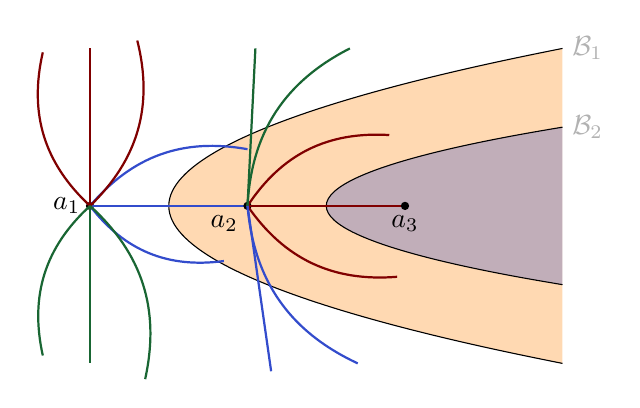
\begin{tikzpicture}[rotate=270]
      \draw [fill opacity=0.3, fill=morange] (2, 0) parabola bend (0, -5) (-2, 0) node [right] {$\mathcal{B}_1$};
      \draw [fill opacity=0.3, fill=mblue] (1, 0) parabola bend (0, -3) (-1, 0) node [right] {$\mathcal{B}_2$};

      \node [circ] at (0, -6) {};
      \node [left] at (0, -6) {$a_1$};

      \draw [thick, mblue] (0, -6) -- (0, -4);
      \draw [thick, mblue] (0, -6) edge [bend left] (-0.72, -4);
      \draw [thick, mblue] (0, -6) edge [bend right] (0.7, -4.3);

      \draw [thick, mred] (0, -6) -- (-2, -6);
      \draw [thick, mred] (0, -6) edge [bend left] (-1.95, -6.6);
      \draw [thick, mred] (0, -6) edge [bend right] (-2.1, -5.4);

      \draw [thick, mgreen] (0, -6) -- (2, -6);
      \draw [thick, mgreen] (0, -6) edge [bend right] (1.9, -6.6);
      \draw [thick, mgreen] (0, -6) edge [bend left] (2.2, -5.3);

      \node [circ] at (0, -4) {};
      \node [anchor = north east] at (0, -4) {$a_2$};

      \draw [thick, mred] (0, -4) -- (0, -2);
      \draw [thick, mred] (0, -4) edge [bend left] (-0.9, -2.2);
      \draw [thick, mred] (0, -4) edge [bend right] (0.9, -2.1);

      \draw [thick, mgreen] (0, -4) edge [bend left] (-2, -2.7);
      \draw [thick, mgreen] (0, -4) -- (-2, -3.9);

      \draw [thick, mblue] (0, -4) edge [bend right] (2, -2.6);
      \draw [thick, mblue] (0, -4) -- (2.1, -3.7);

      \node [circ] at (0, -2) {};
      \node [below] at (0, -2) {$a_3$};
    \end{tikzpicture}
  \end{center}
  We obtain a sequence $\{a_1, a_2, \cdots\}$ and a sequence of colours $\{c_1, c_2, \cdots\}$ such that $c(a_i a_j) = c_i$, for $i < j$.

  Now again by the pigeonhole principle, since there are finitely many colours, there exists an infinite subsequence $c_{i_1}, c_{i_2}, \cdots$ that is constant. Then $a_{i_1}, a_{i_2}, \cdots$ is an infinite monochromatic set, since all edges are of the colour $c_{i_1} = c_{i_2} = \cdots$. So we are done.
\end{proof}
Note that this theorem is highly non-constructive. Not only does it not give us the infinite monochromatic set; it doesn't even tell us what the colour is.

Note also that in the proof, we did not obtain the infinite monochromatic set in one go. Instead, we had to first pass through that intermediate structure, and then obtain an infinite monochromatic set from that. This is a common feature in many proofs in Ramsey theory, and in many cases we have to pass through even more intermediate substructures.

This theorem looks rather innocuous, but it has many interesting applications.
\begin{cor}[Bolzano-Weierstrass theorem]
  Let $(x_i)_{i \geq 0}$ be a bounded sequence of real numbers. Then it has a convergent subsequence.
\end{cor}

\begin{proof}
  We define a colouring $c: \N^{(2)} \to \{\uparrow, \downarrow\}$, where
  \[
    c(ij) =
    \begin{cases}
      \uparrow & x_i < x_j\\
      \downarrow & x_j \leq x_i
    \end{cases}
  \]
  Then Ramsey's theorem gives us an infinite monochromatic set, which is the same as a monotone subsequence. Since this is bounded, it must convergence.
\end{proof}

Now a natural question to ask is --- what happens when we have infinitely many colours? Clearly an infinite monochromatic subset cannot be guaranteed, because we can just colour all edges with different colours. Thus, we can ask a different question --- can we find an $X$ such that \emph{either} $c|_{X}$ is monochromatic, \emph{or} $c|_{X}$ is injective. It turns out this is not quite true, but something very like this is true.

\section{Ramsey theory on the integers}
\section{Partition Regularity}
\section{Topological Dynamics}

\printindex
\end{document}
